\documentclass[12pt, git, final]{rureport}


\begin{document} % this tells the compiler that it is time to make
                 % text to print instead of just getting ready.
\maketitle  % make a title page from the Title, Date, and Author

%\fxnote{skoða titil á skýrslu, sbr. forsíðu}

%\section*{Errata} %%section* avoids putting a number 
%
\section{Inngangur} % sections break up the document into pieces
Himingeimurinn er fyrir mörgum jafn áhugaverður og hann er stór. Mannkynið hefur spáð mikið í himintunglum ásamt öðrum fyrirbærum út í hinum viðamikla geimi frá örófi alda, þau hafa jafnvel í öfgafullum tilfellum verið orsakavaldur styrjalda. Af því hópurinn deilir sömu hrifningu á himinhvolfinu, var ákveðið að ná í gögn um sólmyrkva jarðar, stríð og átök sem herjað hafa á jörðina ásamt vopnasölu út um heim allan og setja upp í gagnagrunn. 

Fyrst og fremst vildi hópurinn skoða hvernig átök heimsins dreifast niður á jörðina, hversu oft og hvar lenda sólmyrkvarnir á jörðina á hverju ári og hvort það sé möguleiki á fylgni milli fjölda sólmyrkva og fjölda stríðsátaka. Þessir útgangspunktar verða skoðaðir nánar og þeim gerðir frekari skil í niðurstöðunum.  
\section{Framkvæmd}
\subsection{Hnötturinn}
Við gerð hnattarins var notast við Basemap \cite{basemap} sem er viðbót við matplotlib. Til að fá hnöttin raunverulegri var notast við bluemarble fallið sem er að finna í Pillow \cite{pillow} pakkanum en það tekur myndir frá NASA \cite{bluemarble} og varpar þeim á hnöttinn. Notast var við gögn úr gagnagrunninum til að fá hnit sólmyrkvana frá 1901-2100 og til að herma eftir snúningi jarðarinnar voru búnar til 180 myndir á tveggja lengdargráðu fresti, en hægt er að skeyta þeim saman í hreyfimynd eða myndband eftir henntisemi notanda með MoviePy pakkanum \cite{moviepy}.
 
%\subsection{Myndrænt notendaviðmót}



\section{Aðferð}
\subsection{Hönnun}
Við hönnun á GUI þá var notast við Qt4 Designer \cite{qt4}. Ákveðið var að hafa glugga sem biður notanda um upplýsingar um gagnagrunn (sjá mynd \ref{fig:logScreen}). Glugginn hefur tvískiptan tilgang, annars vegar er hægt að slá inn upplýsingar til að búa til gagnagrunninn ef hann er ekki til staðar í tölvunni með því að ýta á 'Populate DB' hnappinn. Hins vegar er hægt að tengjast fyrirfram tilbúnum gagnagrunni með því að ýta á ok hnappinn. Þegar notandi velur að búa til gagnagrunn, keyrir forritið populate\_sql.py sem býr til gagnagrunninn, allar töflurnar og fyllir þær. Notandinn þarf þó að vera búinn að fylla út alla dálka á fyrsta spretti glugganum og passa að nafnið á nýja gagnagrunninum sé ekki frátekið, en ef nafnið er frátekið kemur villumelding.

Forritið lætur notandann vita hvort tenging hafi tekist (sjá mynd \ref{fig:logsucces}). Eftir það sprettur upp aðalgluggi forritsins(sjá mynd \ref{fig:openScreen}), sem er í grunninn heimskort með tímastiku fyrir neðan. Kortið sínir einnig 4 dálka sem sýna ástand viðkomandi árs, en hann er útskírður  í kafla \ref{virkni}. Keyrsluskráin hefur tvískipta virkni, annars vegar að teikna staðseningar sem punkta inná kort sem hægt er að smella á og að tala við gagnagrunninn. Ef smellt er á staðsetningu, nær forritið í allar viðeigandi upplýsingar og birtir í viðkomandi dálkum.
 

\subsection{Gögn}
Fyrst var farið á veraldarvefin og leitað að gögnum sem hægt væri að vinna með, gögnin voru fundin á síðu hjá NASA \cite{Eclipse}, Stockholm international peace research institution \cite{weapon} og Háskólanum í Uppsölum í Svíþjóð \cite{conflict}. Gögnin voru tekin inn á csv formi, þau hreinsuð í python og unnið með þau sem Pandas Dataframes áður en þau voru flutt inn í gagnagrunninn sjálfan. Þegar kom að því að túlka hnitin var stuðst við pygeocoder pakkann \cite{geocoder}. Pakkinn tekur við hnitum og gefur heiti viðkomandi lands eða öfugt.





\subsection{Virkni forrits}\label{virkni}
Eftir að notandi er búinn að tengjast gagnagrunni getur hann skoðar ýmsar upplýsingar út frá árum. Það er hægt að hreyfa stiku til að fá ákveðið ár eða slá inn ártalið til að fá viðkomandi upplýsingar um hvað gerðist á því ári. Upplýsingarnar skila sér svo á kortinu sem er á upphafskjánnum og það birtast upplýsingar í dálkum hægra megin við kortið. 

Takki undir grafi gerir notandanum kleift að skipta um tegund korts, annars vegar tvívítt kort og hins vegar hnattlíkan. Við hlið takkans eru svo tveir gátreitir sem stjórna því hvaða upplýsingar birtast á kortinu.


\section{Niðurstöður}\label{nidurstodur}

Þegar staðsetningar sólmyrkvanna eru teiknaðar á hnöttinn sést að hringir myndast á breiddargráðum 60$^{\circ}$-75$^{\circ}$ bæði á norður- (sjá mynd \ref{fig:3DNP}) og suðurhveli jarðar (sjá mynd \ref{fig:3DSP}) og sú lína spannar ca. 43.6\% af öllum sólmyrkvunum sem hafa verið á jörðinni frá tímabilinu 1901 - 2100. Hægt er að sjá að á þeim svæðum þar sem sólmyrkvarnir mynda þéttan kjarna eru mun færri stríð, sbr. 60$^{\circ}$-75$^{\circ}$N og S.

Einnig er hægt að sjá ef vel er rýnt í mynd \ref{fig:3DNP} að nær engir sólmyrkvar eru frá mið-Asíu, niður með mið-austurlöndunum og alveg inn í miðja Afríku. Einnig er það svæðið sem er með hæsta þéttleika átaka ef öll gögn gagnasafnsins eru teiknuð upp í einu. Út frá þessum gögnum er því hægt að draga eftirfarandi huglægt álit: því fleiri átök á landsvæði, því færri sólmyrkvar. \textbf{Always stay on the dark side of life !}
\pagebreak

\begin{figure}
	\centering
	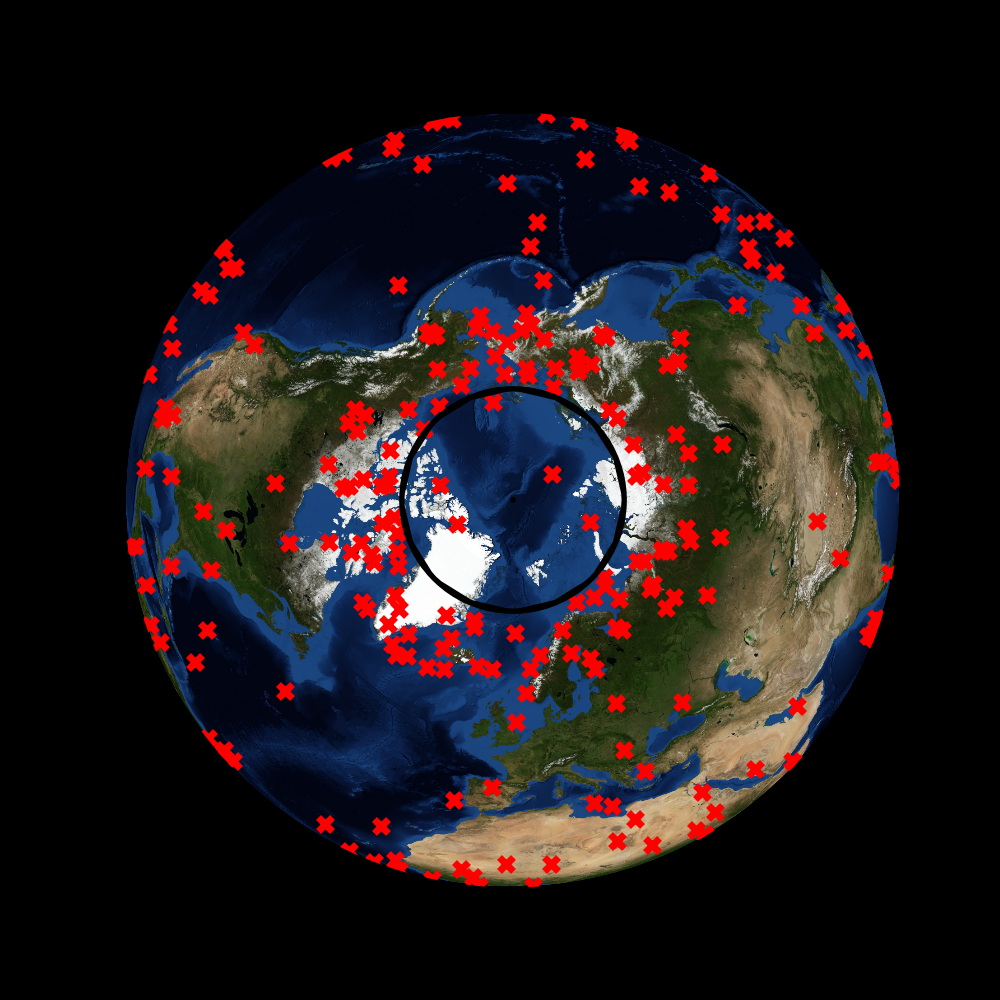
\includegraphics[width=10cm]{3DNP.png}
	\caption{Sólmyrkvarnir séð frá Norður pólnum}
	\label{fig:3DNP}
\end{figure}

\begin{figure}
	\centering
	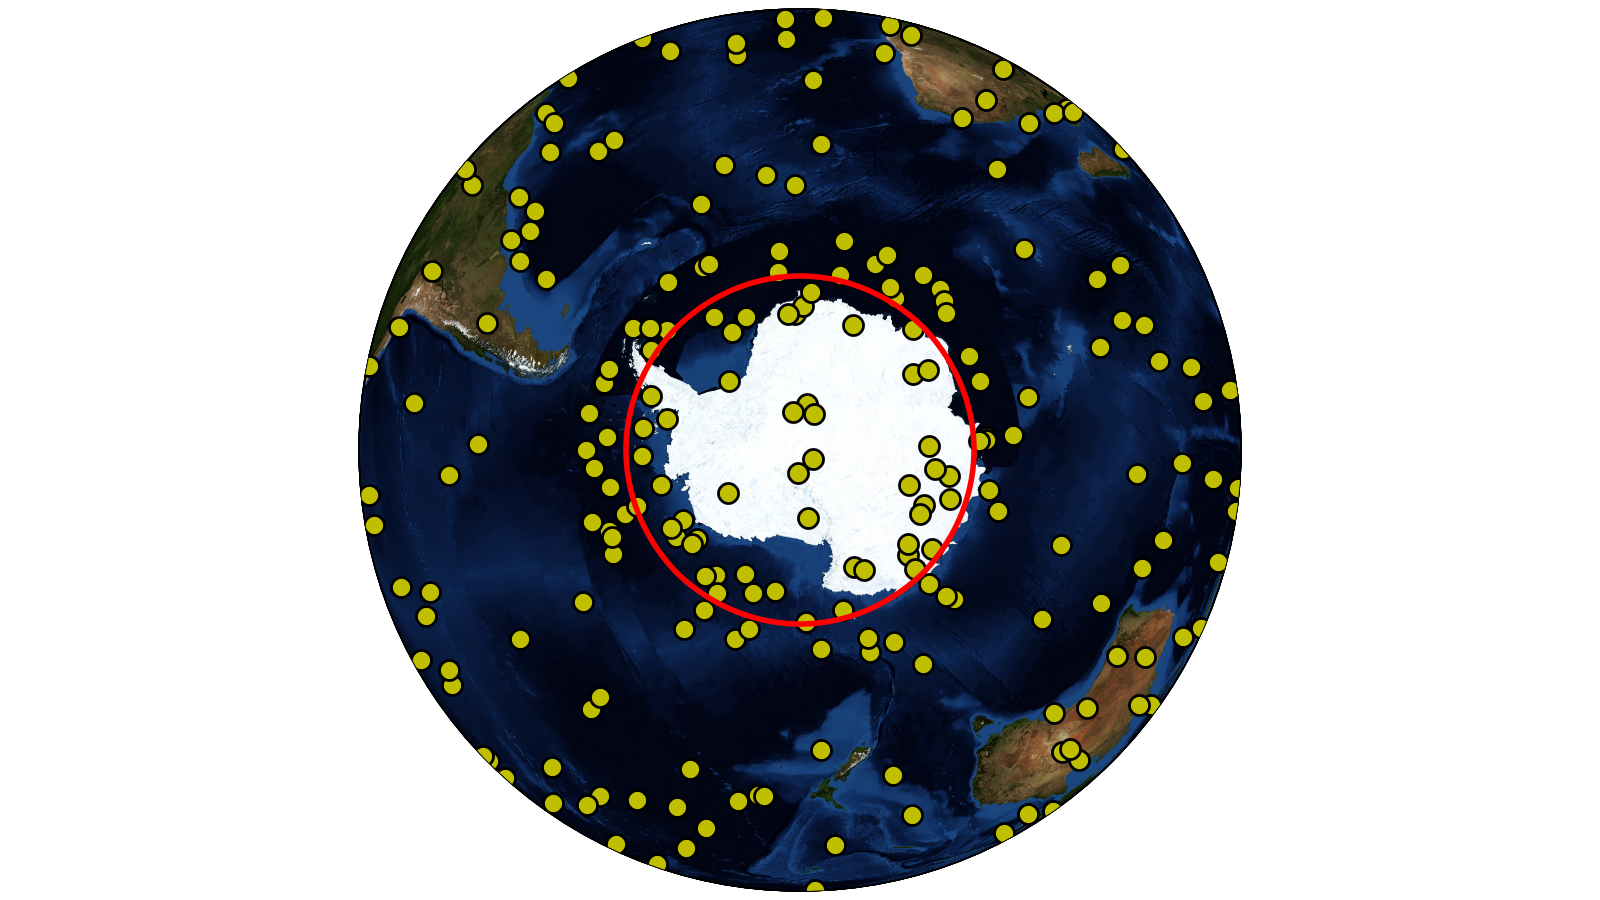
\includegraphics[width=10cm]{3DSP.png}
	\caption{Sólmyrkvarnir séð frá Suður pólnum}
	\label{fig:3DSP}
\end{figure}

\begin{figure}
	\centering 
	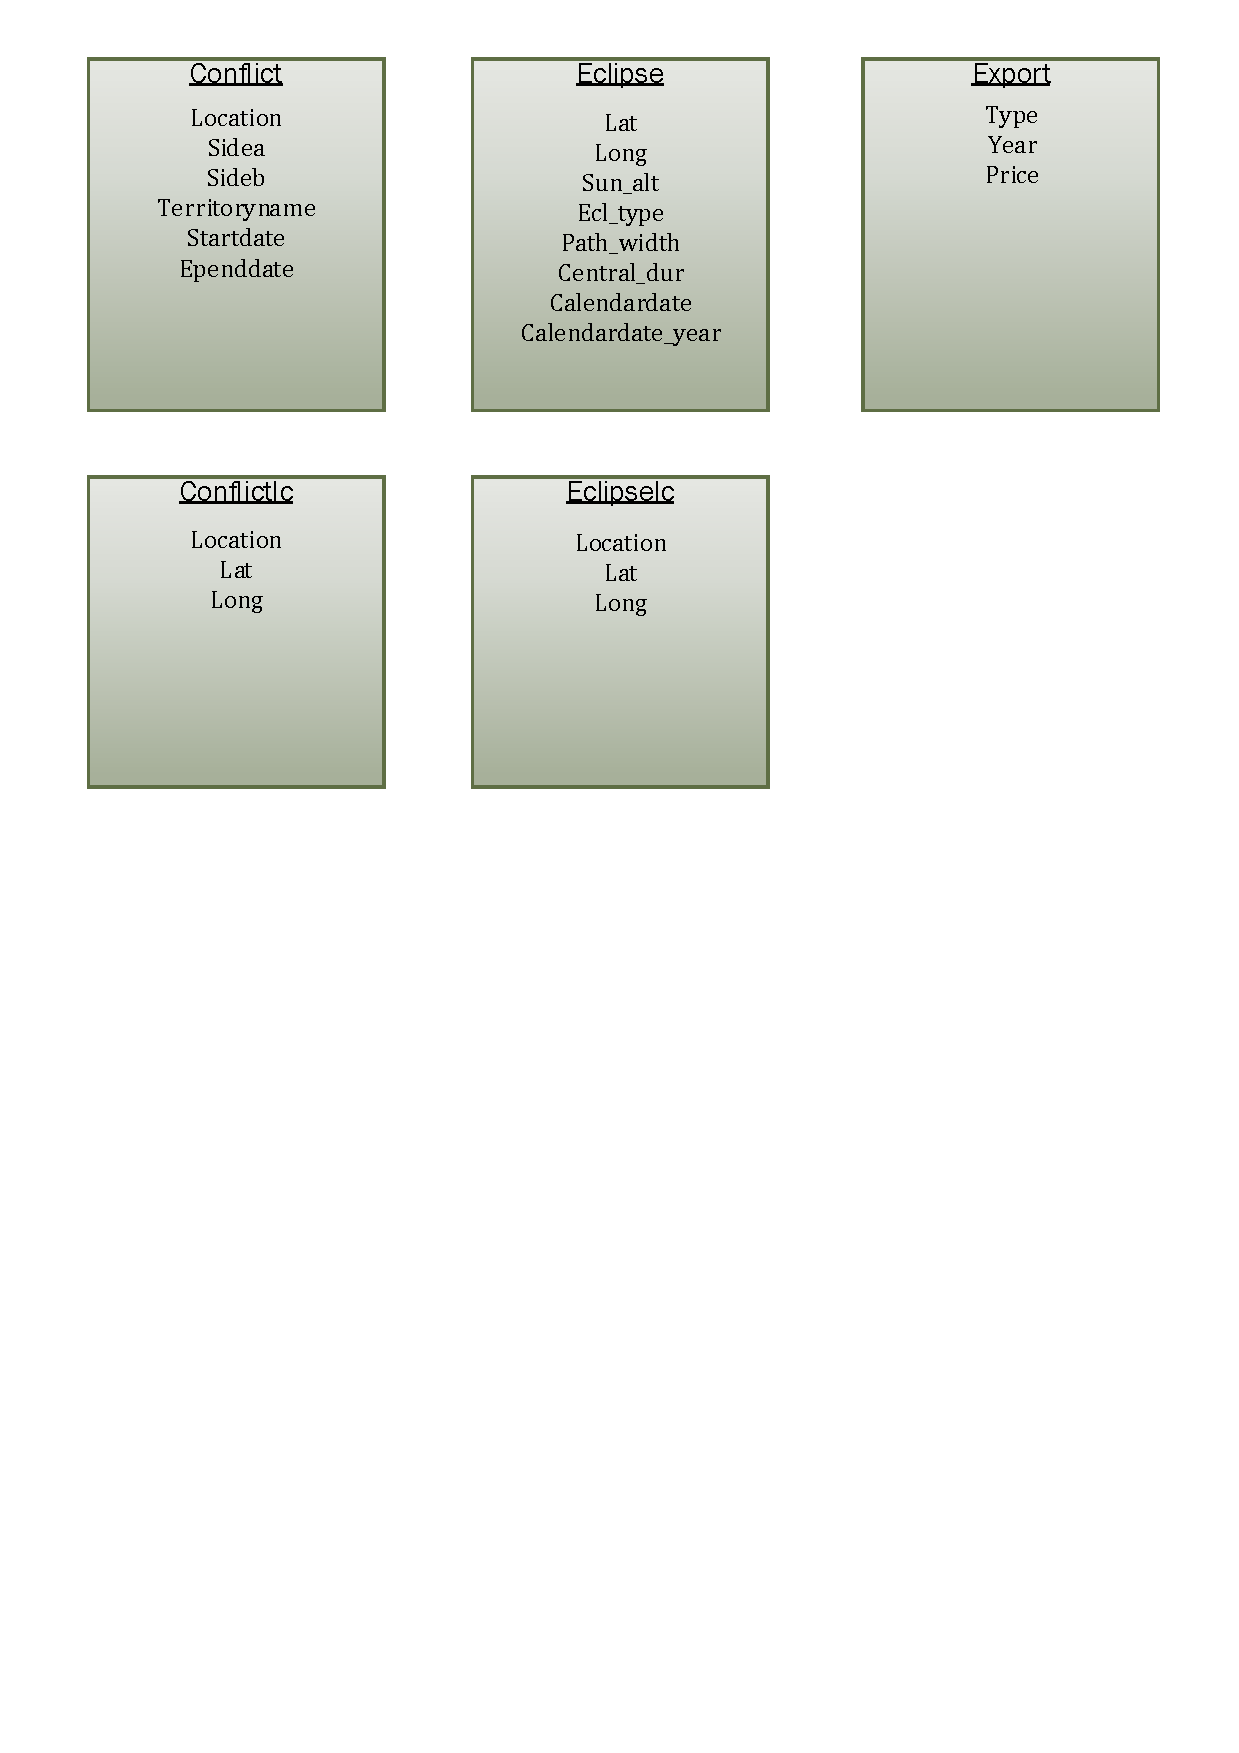
\includegraphics[width = 18cm]{dataSchemaKynn.pdf}
	\caption{Database schema \label{fig:dataschema}}
\end{figure} 
%
\begin{figure}
	\centering 
	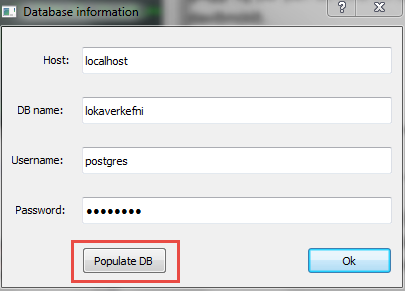
\includegraphics[width = 8cm]{logInScreen.png}
	\caption{Innskráningar glugginn \label{fig:logScreen}}
\end{figure} 

\begin{figure}
	\centering 
	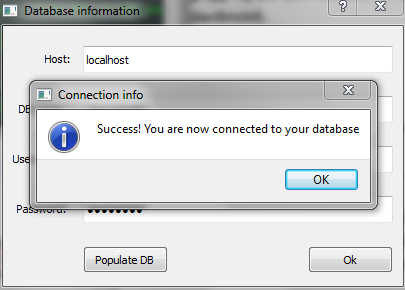
\includegraphics[width = 8cm]{logInSuccess.png}
	\caption{Staðfestingar gluggi á innskráningu \label{fig:logsucces}}
\end{figure} 

\begin{figure}
	\centering 
	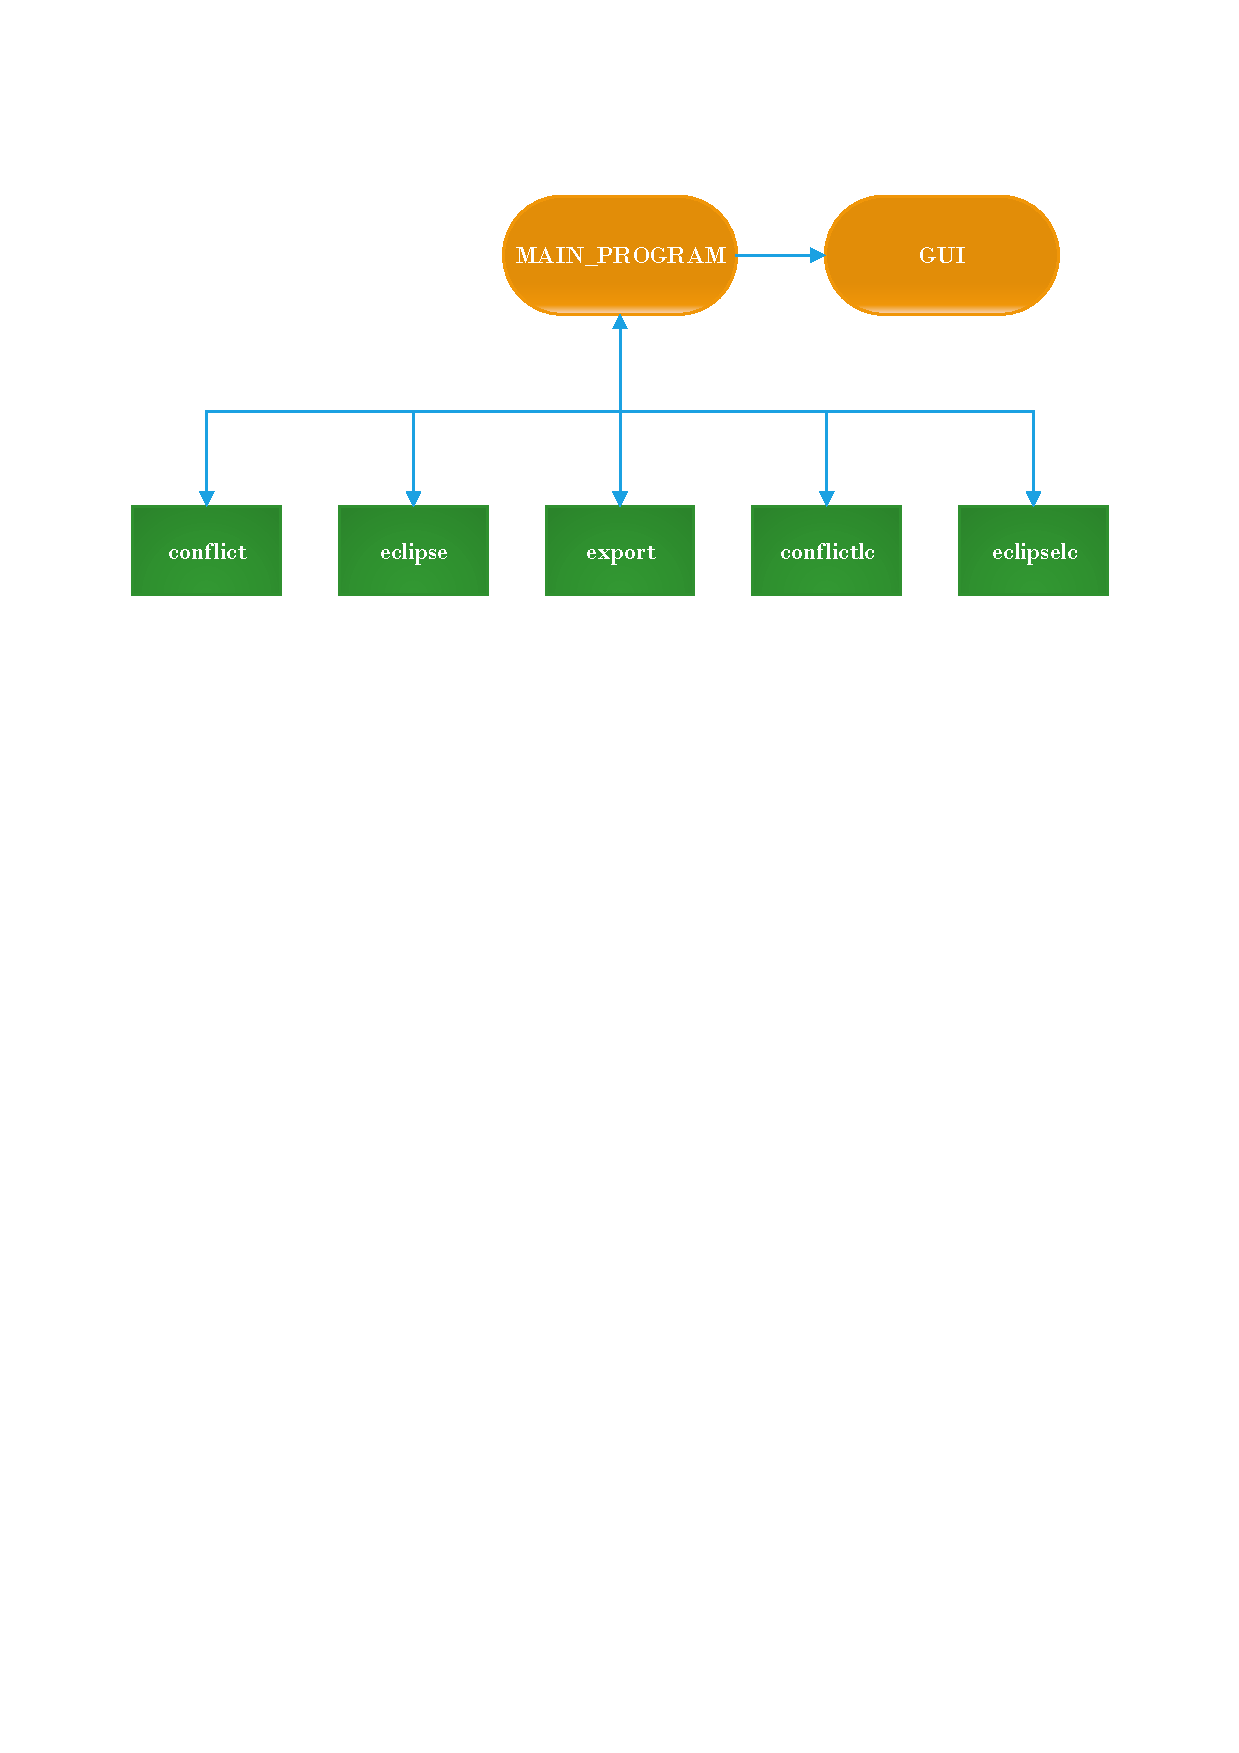
\includegraphics[width = 14cm,trim = 0pt 19cm 0pt 3cm, clip]{ufo.pdf}
	\caption{Staðfestingar gluggi á innskráningu \label{fig:diagram}}
\end{figure}

\begin{figure}[t]
	\centering 
	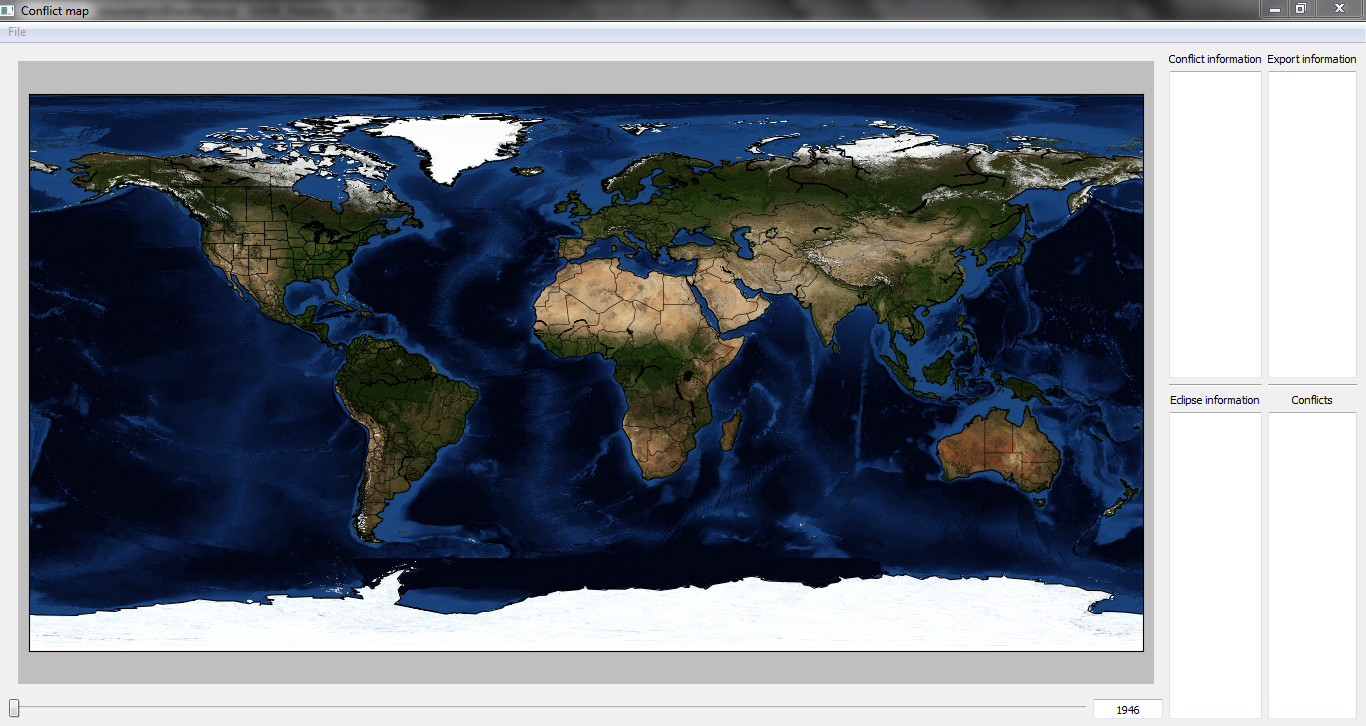
\includegraphics[width = 18cm]{openScreen.png}
	\caption{Aðalgluggi \label{fig:openScreen}}
\end{figure} 
\begin{figure}[t]
	\centering 
	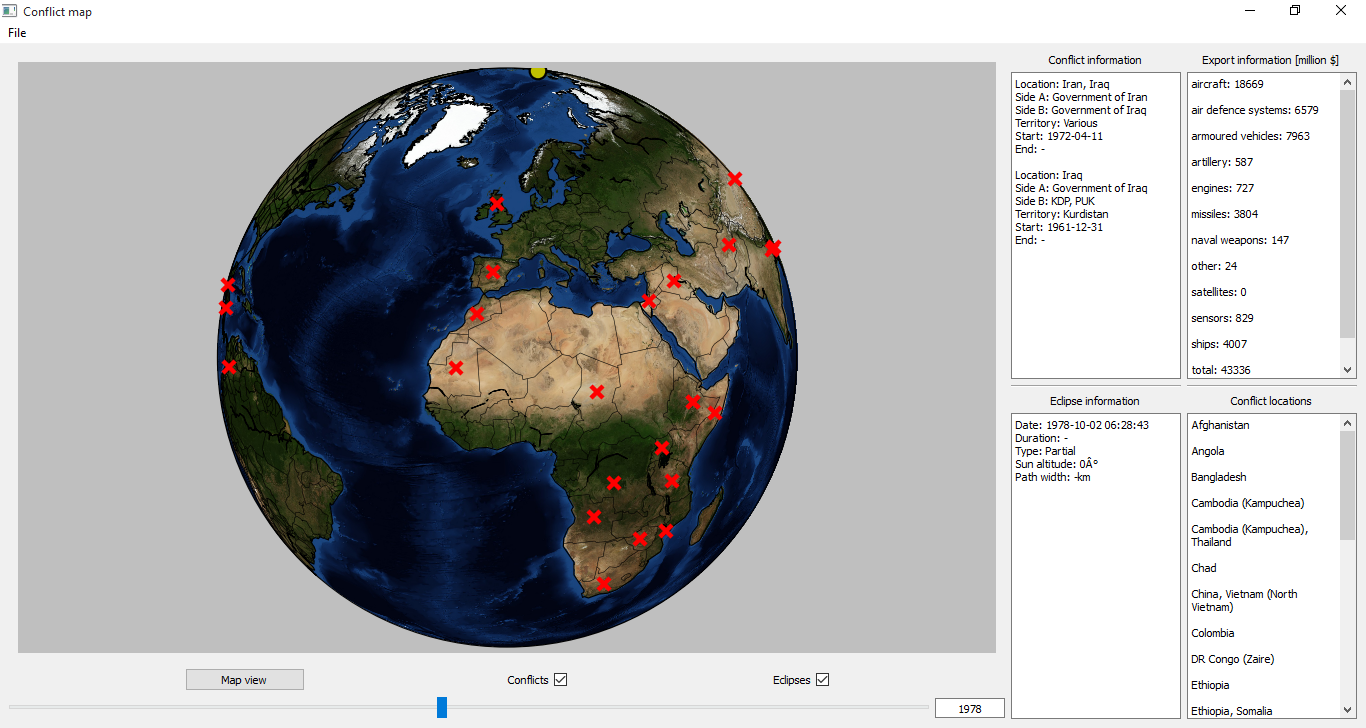
\includegraphics[width = 18cm]{openScreen_globe.png}
	\caption{Aðalgluggi \label{fig:openScreen_globe}}
\end{figure} 

\clearpage

\printbibliography

\end{document} % this tells the compiler that we are done

% These are variables for the editor Emacs
%%% Local Variables: 
%%% TeX-command-BibTeX: biber
%%% mode: latex
%%% TeX-master: t
%%% End:
